\chapter{Vehicular networks}
\label{cha:VN}
\section{Introduction to vehicular networks}
A Mobile Ad-hoc NETwork (MANET) \cite{abolhasan2004review} is defined as a system of mobile nodes, each connected by a wireless connection which can form a graph of an arbitrary structure. These nodes can move independently in every direction or follow a path.
Ad-hoc networks can be built on the spot and used in different kind of scenarios because they do not need a specific infrastructure. The growth of wireless communications led this topic to be one of the most important field of research from the middle of the 1990s.\vskip 1em
A particular case of MANETs are the \textit {Vehicular Ad hoc NETworks} (VANETs), which are a form of wireless ad hoc networks where nodes are vehicles equipped with communication devices that allow them to exchange messages with each other.
In VANETs there are two types of communication: Vehicle-to-Vehicle communication (V2V) and Vehicle-to-Infrastructure communication (V2I) where vehicles exchange messages with roadside network infrastructures (RSU). For example, \Cref{fig:vanet} \cite{Sanguesa2015vanet} shows the possible connections that can occur between nodes in a VANET.
\begin{figure}[H]
    \centering
    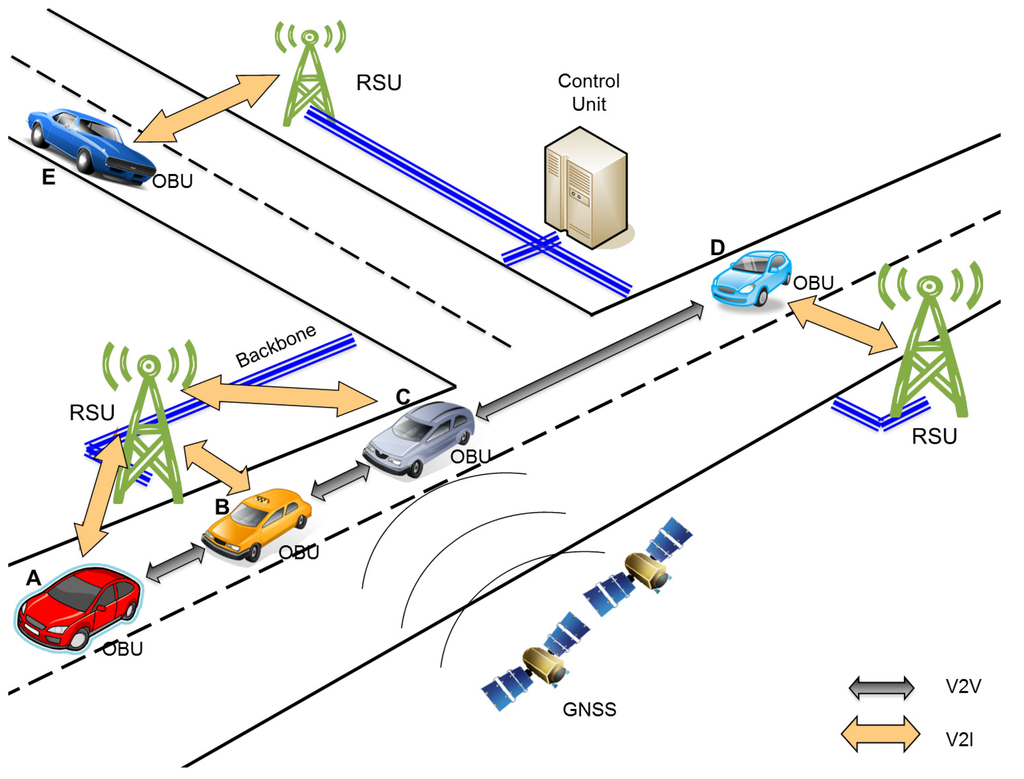
\includegraphics[width=0.6\textwidth]{fig/vanet.png}
    \caption{A representation of V2I and V2V connections}
    \label{fig:vanet}
\end{figure}
In the early 2000s VANETs were seen as an application of MANET principles but they soon became a research field on its own. Being the basis for what we call Inter-Vehicle-Communication \cite{ivc} (IVC), today the term is still somewhat synonymous with IVC, but it focuses on spontaneously created ad hoc networks and less on using pre-deployed infrastructure like RSUs.\vskip 1em
Several major automobile manufacturers have already begun to invest in real inter-vehicle networks and  have joined to create a non-profit organization called \textit {Car2Car Communication Consortium} (C2CCC) \cite{c2ccc} in order to increasing road traffic safety and efficiency by means of IVC.
\section{Application}
\label{sec:appl}
Here the concepts of operation for applications used in VANET systems are presented.
Applications can be classified into two main categories: vehicle-to-vehicle and infrastructure-to-vehicle applications.
Although most implementations of V2V applications only warn the driver of imminent collision or danger, the use of autonomous vehicle actions like braking or steering can be an important field of research in future systems.
\subsection{V2I applications}\vskip 1em
\label{subsec:V2I}
\textbf {Intersection violation warning} \vskip 1em
The intersection violation warning (IVW) application warns drivers when the violation of a red light seems imminent. A roadside unit co-located with a traffic light controller will broadcast information about location, light phase, light timing and intersection geometry to vehicles which are going to approach the intersection.
Vehicles then can compare this information with their trajectories and determine whether a signal violation is imminent. If so, the driver will be alerted and a signal is sent to the traffic light and surrounding vehicles to inform that a warning has been issued. \Cref{fig:ivwsafety}  \cite{hartenstein2010vanet} shows the violation of a red light.
\begin{figure}[H]
    \centering
    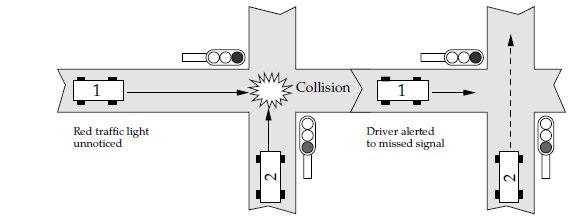
\includegraphics[width=0.75\textwidth]{fig/Ivw.png}
    \caption{Without IVW the driver will not be notified and so an accident can occur, while with IVW the driver will be notified and so he can slow down.}
    \label{fig:ivwsafety}
\end{figure}
\subsection{V2V applications}\vskip 1em
\label{subsec:V2V}
\textbf{Electronic Brake Warning} \vskip 1em
The electronic brake warning \cite{Szczurek_EBW}(EWB) application alerts driver when a preceding vehicle performs a hard braking maneuver. The application is particularly useful when the view is blocked by other vehicles. When a vehicle brakes sharply, it produces a message that is sent to surrounding vehicles indicating it is undergoing hard braking. When the message is received, the system has to decide whether the message is relevant or irrelevant such as message from vehicles travelling behind or in the opposite direction. \vskip 1em
\textbf{Vehicle stability warning} \vskip 1em
The vehicle stability warning (VSW) application alerts the driver of preceding vehicles that have used the \emph{Stability Control System}. This will allow following vehicles to prepare for upcoming hazardous condition and so adjust their own VSW system. Otherwise, the application can alert drivers to keep attention on upcoming road condition by suggesting eyes forward or both hands on steering wheel.
\newpage
\textbf{Traffic Management} \vskip 1em
Traffic management is utilized by authorities in both V2I and V2V application. Authorities can use data from an RSU, which can receive information about position from surrounding vehicles, in order ease traffic flow and provide a real time response to congestion. They may change traffic rules according to specific situation such as bad weather. While these applications are almost based on V2I communication,  in \cite{gupte2012vehicular} V2V communication is used as a  possible solution for Intelligent and Autonomous Traffic Management, where vehicles can change their route according to the neighbors routes.
\section{Communication technology}
\label{sec:com_tech}
A wide variety of short radio technologies can be used for IVC such as Bluetooth, Zigbee or optical link. However the IVC community has developed an IEEE 802.11 derived standard specific to vehicular called IEEE 802.11p.\vskip 1em
IEEE 802.11p is one of the recent approved amendments to the IEEE 802.11 standard to enable wireless access in vehicular environments (WAVE). It appended some enhancements to the latest version of 802.11 that required to support applications of Intelligent Transportation Systems (ITS) \cite{eichler2007performance}. This includes data exchange between high-speed vehicles and between the vehicles and the roadside infrastructure in the licensed ITS band. \\
The development of the IEEE802.11p standard originates from the allocation of the Dedicated Short Range Communications (DSRC) spectrum band.
In 1999, the U.S. Federal Communication Commission (FCC) allocated in the U.S. \SI{75}{\MHz} of DSRC spectrum at \SI{5.9}{\GHz} to be used exclusively for ITS applications. The primary goal was to develop applications for safety and traffic enhancement. Private services were also permitted in order to decrease the deployment costs and encourage the adoption of DSRC technologies.\\
Out of \SI{75}{\MHz} spectrum, \SI{5}{\MHz} is reserved as the guard band  and seven \SI{10}{\MHz} channels are defined as shown in \Cref{fig:dsrc_spectrum} \cite{sahoo2014svanet}.
\begin{figure} [H]
    \centering
    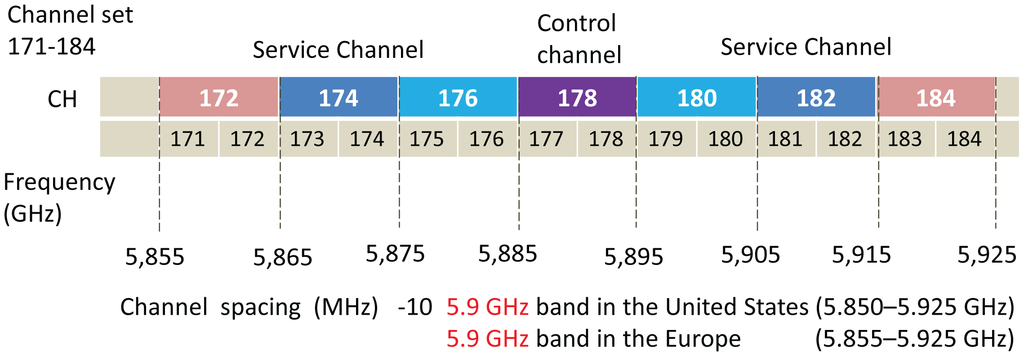
\includegraphics[width=0.70\textwidth]{fig/dsrc_spectrum.png}
    \caption{The DSRC Frequency Allocation in US}
    \label{fig:dsrc_spectrum}
\end{figure}
The seven channels are divided into 1 control channel (CCH) and 6 service channels (SCHs). The CCH is restricted to high-priority short message or data management and it is the only one shared between all WAVE devices. The first and the last channels of the spectrum are reserved for "public safety applications involving safety of life and property" \cite{fcc}.
\begin{figure} [H]
    \centering
    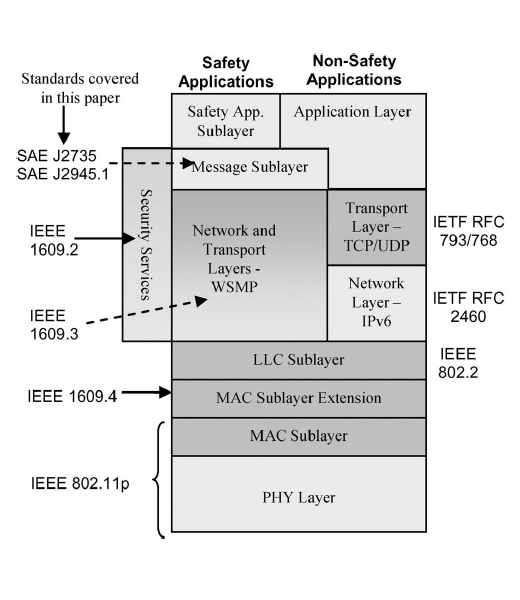
\includegraphics[width=0.50\textwidth]{fig/dsrc.png}
    \caption{DSRC architecture.}
    \label{fig:dsrc}
\end{figure}
\subsection{DSRC protocol stack}
As shown in \Cref{fig:dsrc} the DSRC architecture incorporates a number of protocols and corresponding standards. IEEE 802.11p provides the basic radio standard for DSRC. IEEE 802.11p is limited by the scope of IEEE 802.11, which is a MAC and PHY layer standard meant for single physical channel operation. The DSRC multi-channel setup and the operational concepts are taken care of by the upper layer IEEE 1609.x\cite{CJD_IEEE}.:
\begin{itemize}
	\item \emph{1609.1} Resource Manager: This standard provides a resource manager for WAVE, allowing communication between remote applications and vehicles.;
	\item \emph{1609.2} Security Services for Applications and Management Messages;
	\item \emph{1609.3} Networking Services: This standard addresses network layer issues in WAVE;
	\item \emph{1609.4} Multi-channel Operation: This standard deals with communications through multiple channels.
\end{itemize}
In particular, the IEEE 1609.3 \cite{1609.3} standard covers the WAVE connection setup and management. The IEEE 1609.4 \cite{1609.4} standard sits right on top of the IEEE 802.11p and enables operation of upper layers across multiple channels, without requiring knowledge of PHY parameters.\vskip 1em
The IEEE 802.11p physical layer is OFDM-based, and quite similar to the IEEE 802.11a physical layer design. The main difference is in the overall bandwidth used, which is \SI{10}{\MHz} for IEEE 802.11p instead of the 20 MHz of IEEE 802.11a. \vskip 1em
The IEEE 802.11p standard is meant to:
\begin{itemize}
    \item Describe the functions and services required by
WAVE-conformant stations to operate in a rapidly
varying environment and exchange messages without
having to join a Basic Service Set (BSS), as in the
traditional IEEE 802.11 use case.
    \item Define the WAVE signaling technique and interface
functions that are controlled by the IEEE 802.11
MAC.
\end{itemize}
\newpage
